%What is a variogram, its application, why not yet parallel, comparison to particle simulation
%Note on how this will actually be used in research
%How we tested for correctness


The field of geostatistics strives to characterize the spatial heterogeneity found in the physical world in terms of probability and statistics. A common method to represent how values of a field are correlated over space is called a variogram. The variogram is a function of distance between points in space and describes the increase in variance between points as distance grows. The shape of a variogram is highly informative for gauging the heterogeneity of a spatial field. For example, the near-origin slope of the variogram indicates if values change smoothly or sharply across the field. 

One important application of variograms is in groundwater modeling. Measuring hydraulic properties of aquifers is difficult because most methods involve drilling into the subsurface, which is expensive and destructive. Measurements are often scarce and modelers have traditionally averaged their sparse data to assign constant values in their numerical models, however studies have shown that certain subsurface processes are highly dependent on aquifer heterogeneity. Variograms are used to construct covariance matrices of multi-normal distributions which are sampled to create realizations of random heterogeneous fields. An ensemble of these random fields can be used to study subsurface processes in a stochastic fashion.      

To estimate a field site's variogram, measurements are used to construct an empirical variogram: 
\begin{equation}
\hat{\gamma}(h)=\frac{1}{2|N(h)|}\sum_{(i,j)\in N(h)} |z_i-z_j|^2
\end{equation}
where $h$ is distance between two points in space ($i$ and $j$), the value of the field at point $i$ is $z_i$, $N(h)$ is the group of pairs of points separated by distance $h$, and $|N(h)|$ is the number of pairs in the group. Geostatistical software packages exist to convert spatial data measurements into empirical variograms already, but they are designed for small data sets. Since most field site's only have between $10^1 - 10^3$ data points, the straight-forward $O(n^2)$ algorithm for calculating the empirical variogram is computationally feasible. However, current research is being conducted with three-dimensional aquifer analogs to understand realistic heterogeneities given fully known domains. Figure~\ref{fig:herten} is a visualization of such a data set and it contains $8.96\times 10^6$ data points which creates $4\times 10^13$ pairs to consider in the empirical variogram calculation. Using the traditional geostatistical packages on a personal computer for this data set would require an unreasonable amount of time (on the order of weeks). Thus, we chose to pursue the empirical variogram calculation for large data sets as our project.   

\begin{figure}[!htbp]
   \centering
   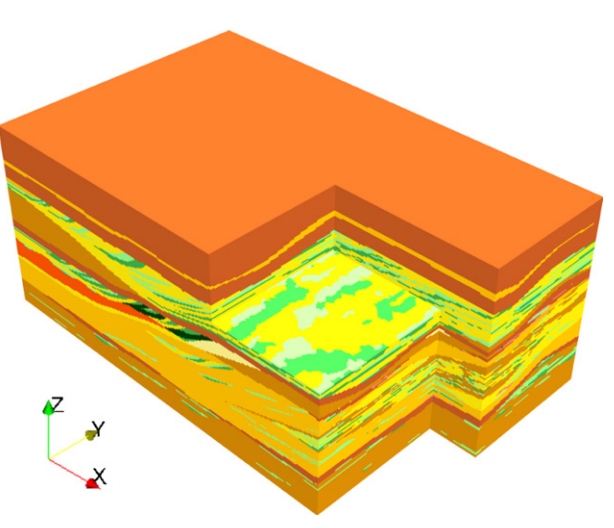
\includegraphics{./fig/herten.png} % requires the graphicx package
   \caption{A visualization of a three-dimensional aquifer analog. The domain covers 16x10x7m at 5cm resolution. The color indicates soil type, which influences groundwater flow and contaminant transport processes. (Copied from \cite{Comunian2011a})}
   \label{fig:herten}
\end{figure}


